% *****************************************************************************************************
% ****************************              SIMPLE EXAMPLE             ********************************
% *****************************************************************************************************

% =======================================================
% =======         HEADER FOR DOCUMENT        ============
% =======================================================
    
    % *********  SPECIFIC FOR THIS BOOK  ********
    \def\ProjectAuthorLink{https://github.com/SoyOscarRH}
    \def\ProjectNameLink{\ProjectAuthorLink/LibroCriptografia}    
    

    % *********   DOCUMENT ITSELF   **************
    \documentclass[12pt, fleqn]{report}                             %Type of doc and size of font and left equations
    \usepackage[margin=1.2in]{geometry}                             %Margins and Geometry pacakge
    \usepackage{ifthen}                                             %Allow simple programming using if - then
    \usepackage[hidelinks]{hyperref}                                %Allow to create hiperlinks and Fuck Firefox
    \usepackage{pdfpages}                                           %Allow us 'import' PDF's
    \hypersetup{pageanchor=false}                                   %Solve 'double page 1' warnings in build :v
    \setlength{\parindent}{0pt}                                     %Eliminate ugly indentation
    \author{Oscar Andrés Rosas}                                     %Who I am

    % *********   LANGUAJE    *****************
    \usepackage[spanish]{babel}                                     %Please allow me to type in spanish
    \usepackage[utf8]{inputenc}                                     %Lets use UFT-8
    \usepackage[T1]{fontenc}                                        %Allow for better font support
    \usepackage{textcmds}                                           %Allow us to use quoutes
    \usepackage{changepage}                                         %Allow us to use identate paragraphs
    \usepackage{anyfontsize}                                        %All the sizes for fonts wiiiii!

    % *********   MATH AND HIS STYLE  *********
    \usepackage{ntheorem, amsmath, amssymb, amsfonts}               %All fucking math, I want all!
    \usepackage{mathrsfs, mathtools, empheq}                        %All fucking math, I want all!
    \usepackage{cancel}                                             %Negate symbol
    \usepackage{centernot}                                          %Allow me to negate a symbol
    \decimalpoint                                                   %Use decimal point

    % *********   GRAPHICS AND IMAGES *********
    \usepackage{graphicx}                                           %Allow to create graphics
    \usepackage{float}                                              %For images
    \usepackage{wrapfig}                                            %Allow to create images
    \graphicspath{ {Graphics/} }                                    %Where are the images :D

    % *********   LISTS AND TABLES ***********
    \usepackage{listings, listingsutf8}                             %We will be using code here
    \usepackage[inline]{enumitem}                                   %We will need to enumarate
    \usepackage{tasks}                                              %Horizontal lists
    \usepackage{longtable}                                          %Lets make tables awesome
    \usepackage{booktabs}                                           %Lets make tables awesome
    \usepackage{tabularx}                                           %Lets make tables awesome
    \usepackage{multirow}                                           %Lets make tables awesome
    \usepackage{multicol}                                           %Create multicolumns

    % *********   REMOVE SOME ERRORS **********
    \hbadness=10000                                                 %Ignore \vbox and \hbox warings
    \hfuzz=\maxdimen\newdimen\hfuzz                                 %Ignore \vbox and \hbox warings

    % *********   HEADERS AND FOOTERS ********
    \usepackage{fancyhdr}                                           %Lets make awesome headers/footers
    \pagestyle{fancy}                                               %Lets make awesome headers/footers
    \setlength{\headheight}{16pt}                                   %Top line
    \setlength{\parskip}{0.5em}                                     %Top line
    \renewcommand{\footrulewidth}{0.5pt}                            %Bottom line

    \lhead {                                                        %Left Header
        \hyperlink{chapter.\arabic{chapter}}                        %Make a link to the current chapter
        {\normalsize{\textsc{\nouppercase{\leftmark}}}}             %And fot it put the name
    }

    \rhead {                                                        %Right Header
        \hyperlink{section.\arabic{chapter}.\arabic{section}}       %Make a link to the current chapter
            {\footnotesize{\textsc{\nouppercase{\rightmark}}}}      %And fot it put the name
    }

    \rfoot{\textsc{\small{\hyperref[sec:Index]{Ve al Índice}}}}     %This will always be a footer  

    \fancyfoot[L]{                                                  %Algoritm for a changing footer
        \ifthenelse{\isodd{\value{page}}}                           %IF ODD PAGE:
            {\href{https://SoyOscarRH.github.io/}                   %DO THIS:
                {\footnotesize                                      %Send the page
                    {\textsc{Oscar Andrés Rosas}}}}                 %Send the page
            {\href{https://compilandoconocimiento.com}              %ELSE DO THIS: 
                {\footnotesize                                      %Send the author
                    {\textsc{Compilando Conocimiento}}}}            %Send the author
    }
    
    
% =======================================================
% ===================   COMMANDS    =====================
% =======================================================

    % =========================================
    % =======   NEW ENVIRONMENTS   ============
    % =========================================
    \newenvironment{Indentation}[1][0.75em]                         %Use: \begin{Inde...}[Num]...\end{Inde...}
        {\begin{adjustwidth}{#1}{}}                                 %If you dont put nothing i will use 0.75 em
        {\end{adjustwidth}}                                         %This indentate a paragraph
    
    \newenvironment{SmallIndentation}[1][0.75em]                    %Use: The same that we upper one, just 
        {\begin{adjustwidth}{#1}{}\begin{footnotesize}}             %footnotesize size of letter by default
        {\end{footnotesize}\end{adjustwidth}}                       %that's it
    
    \def \Eq {equation}                                             %Stupid Visual studio error
    \newenvironment{MultiLineEquation}[1]                           %Use: To create MultiLine equations
        {\begin{\Eq}\begin{alignedat}{#1}}                          %Use: \begin{Multi..}{Num. de Columnas}
        {\end{alignedat}\end{\Eq}}                                  %And.. that's it!
    
    \newenvironment{MultiLineEquation*}[1]                          %Use: To create MultiLine equations
        {\begin{\Eq*}\begin{alignedat}{#1}}                         %Use: \begin{Multi..}{Num. de Columnas}
        {\end{alignedat}\end{\Eq*}}                                 %And.. that's it!

    \newenvironment{largeEq} {\begingroup \large}{\endgroup}        %Make eq bigger
    \newenvironment{LargeEq} {\begingroup \Large}{\endgroup}        %Make eq bigger
    \newenvironment{HugeEq} {\begingroup \Huge}{\endgroup}          %Make eq bigger!

    % =========================================
    % == GENERAL TEXT & SYMBOLS ENVIRONMENTS ==
    % =========================================
    
    % =====  TEXT  ======================
    \newcommand \Quote              {\qq}                           %Use: \Quote to use quotes
    \newcommand \Over               {\overline}                     %Use: \Bar to use just for short
    \newcommand \ForceNewLine       {$\Space$\\}                    %Use it in theorems for example
    \newcommand \ForceColumnBreak   {\vfill\null\columnbreak}       %Use only in multicols
    \newcommand \Link[2] {\underline{\texttt{\href{#1}{#2}}}}       %Use a link

    % =====  SPACES  ====================
    \DeclareMathOperator \Space     {\quad}                         %Use: \Space for a cool mega space
    \DeclareMathOperator \MegaSpace {\quad \quad}                   %Use: \MegaSpace for a cool mega mega space
    \DeclareMathOperator \MiniSpace {\;}                            %Use: \Space for a cool mini space
    
    % =====  MATH TEXT  =================
    \newcommand \Such           {\MiniSpace | \MiniSpace}           %Use: \Such like in sets
    \newcommand \Also           {\MiniSpace \text{y} \MiniSpace}    %Use: \Also so it's look cool
    \newcommand \Remember[1]    {\Space\text{\scriptsize{#1}}}      %Use: \Remember so it's look cool
    
    % =====  THEOREMS: IN SPANISH :0  ===
    \newtheorem{Theorem}        {Teorema}[section]                  %Use: \begin{Theorem}[Name]\label{Nombre}...
    \newtheorem{Corollary}      {Colorario}[Theorem]                %Use: \begin{Corollary}[Name]\label{Nombre}...
    \newtheorem{Lemma}[Theorem] {Lemma}                             %Use: \begin{Lemma}[Name]\label{Nombre}...
    \newtheorem{Definition}     {Definición}[section]               %Use: \begin{Definition}[Name]\label{Nombre}...
    \theoremstyle{break}                                            %THEOREMS START 1 SPACE AFTER Fuck!

    % =====  LOGIC  =====================
    \newcommand \lIff    {\leftrightarrow}                          %Use: \lIff for logic iff
    \newcommand \lEqual  {\MiniSpace \Leftrightarrow \MiniSpace}    %Use: \lEqual for a logic double arrow
    \newcommand \lInfire {\MiniSpace \Rightarrow \MiniSpace}        %Use: \lInfire for a logic infire
    \newcommand \lLongTo {\longrightarrow}                          %Use: \lLongTo for a long arrow
    \newcommand \lAnd    {\land}                                    %Use: \lAnd ^
    \newcommand \lOr     {\lor}                                     %Use: \lOr or symbol
    \newcommand \lNot    {\neg}                                     %Use: \lNot for negation

    % =====  FAMOUS SETS  ===============
    \DeclareMathOperator \Naturals     {\mathbb{N}}                 %Use: \Naturals por Notation
    \DeclareMathOperator \Primes       {\mathbb{P}}                 %Use: \Primes por Notation
    \DeclareMathOperator \Integers     {\mathbb{Z}}                 %Use: \Integers por Notation
    \DeclareMathOperator \Racionals    {\mathbb{Q}}                 %Use: \Racionals por Notation
    \DeclareMathOperator \Reals        {\mathbb{R}}                 %Use: \Reals por Notation
    \DeclareMathOperator \Complexs     {\mathbb{C}}                 %Use: \Complex por Notation
    \DeclareMathOperator \GenericField {\mathbb{F}}                 %Use: \GenericField por Notation
    \DeclareMathOperator \VectorSet    {\mathbb{V}}                 %Use: \VectorSet por Notation
    \DeclareMathOperator \SubVectorSet {\mathbb{W}}                 %Use: \SubVectorSet por Notation
    \DeclareMathOperator \Polynomials  {\mathbb{P}}                 %Use: \Polynomials por Notation
    \DeclareMathOperator \VectorSpace  {\VectorSet_{\GenericField}} %Use: \VectorSpace por Notation
    \DeclareMathOperator \LinealTransformation {\mathcal{T}}        %Use: \LinealTransformation for a cool T
    \DeclareMathOperator \LinTrans      {\mathcal{T}}               %Use: \LinTrans for a cool T
    \DeclareMathOperator \Laplace       {\mathcal{L}}               %Use: \LinTrans for a cool T

    % =====  CONTAINERS   ===============
    \newcommand{\Set}[1]            {\left\{ \; #1 \; \right\}}     %Use: \Set {Info} for INTELLIGENT space 
    \newcommand{\bigSet}[1]         {\big\{  \; #1 \; \big\}}       %Use: \bigSet  {Info} for space 
    \newcommand{\BigSet}[1]         {\Big\{  \; #1 \; \Big\}}       %Use: \BigSet  {Info} for space 
    \newcommand{\biggSet}[1]        {\bigg\{ \; #1 \; \bigg\}}      %Use: \biggSet {Info} for space 
    \newcommand{\BiggSet}[1]        {\Bigg\{ \; #1 \; \Bigg\}}      %Use: \BiggSet {Info} for space 
        
    \newcommand{\Wrap}[1]           {\left( #1 \right)}             %Use: \Wrap {Info} for INTELLIGENT space
    \newcommand{\bigWrap}[1]        {\big( \; #1 \; \big)}          %Use: \bigBrackets  {Info} for space 
    \newcommand{\BigWrap}[1]        {\Big( \; #1 \; \Big)}          %Use: \BigBrackets  {Info} for space 
    \newcommand{\biggWrap}[1]       {\bigg( \; #1 \; \bigg)}        %Use: \biggBrackets {Info} for space 
    \newcommand{\BiggWrap}[1]       {\Bigg( \; #1 \; \Bigg)}        %Use: \BiggBrackets {Info} for space 

    \newcommand{\Brackets}[1]       {\left[ #1 \right]}             %Use: \Brackets {Info} for INTELLIGENT space
    \newcommand{\bigBrackets}[1]    {\big[ \; #1 \; \big]}          %Use: \bigBrackets  {Info} for space 
    \newcommand{\BigBrackets}[1]    {\Big[ \; #1 \; \Big]}          %Use: \BigBrackets  {Info} for space 
    \newcommand{\biggBrackets}[1]   {\bigg[ \; #1 \; \bigg]}        %Use: \biggBrackets {Info} for space 
    \newcommand{\BiggBrackets}[1]   {\Bigg[ \; #1 \; \Bigg]}        %Use: \BiggBrackets {Info} for space 

    \newcommand{\Generate}[1]   {\left\langle #1 \right\rangle}     %Use: \Generate {Info} <>
    \newcommand{\Floor}[1]      {\left \lfloor #1 \right \rfloor}   %Use: \Floor {Info} for floor 
    \newcommand{\Ceil}[1]       {\left \lceil #1 \right \rceil }    %Use: \Ceil {Info} for ceil
    
    % =====  BETTERS MATH COMMANDS   =====
    \newcommand{\pfrac}[2]      {\Wrap{\dfrac{#1}{#2}}}             %Use: Put fractions in parentesis
    \newcommand{\Sum}           {\displaystyle \sum}                %Use: Sum to big sum
    \newcommand{\Int}           {\displaystyle \int}                %Use: Sum to big integral


    % =========================================
    % ====   LINEAL ALGEBRA & VECTORS    ======
    % =========================================

    % ===== UNIT VECTORS  ================
    \newcommand{\hati}      {\hat{\imath}}                           %Use: \hati for unit vector    
    \newcommand{\hatj}      {\hat{\jmath}}                           %Use: \hatj for unit vector    
    \newcommand{\hatk}      {\hat{k}}                                %Use: \hatk for unit vector

    % ===== MAGNITUDE  ===================
    \newcommand{\abs}[1]    {\left\lvert #1 \right\lvert}           %Use: \abs{expression} for |x|
    \newcommand{\Abs}[1]    {\left\lVert #1 \right\lVert}           %Use: \Abs{expression} for ||x||
    \newcommand{\Mag}[1]    {\left| #1 \right|}                     %Use: \Mag {Info} 
    
    \newcommand{\bVec}[1]   {\mathbf{#1}}                           %Use for bold type of vector
    \newcommand{\lVec}[1]   {\overrightarrow{#1}}                   %Use for a long arrow over a vector
    \newcommand{\uVec}[1]   {\mathbf{\hat{#1}}}                     %Use: Unitary Vector Example: $\uVec{i}

    % ===== FN LINEAL TRANSFORMATION  ====
    \newcommand{\FnLinTrans}[1]{\mathcal{T}\Wrap{#1}}               %Use: \FnLinTrans for a cool T
    \newcommand{\VecLinTrans}[1]{\mathcal{T}\pVector{#1}}           %Use: \LinTrans for a cool T
    \newcommand{\FnLinealTransformation}[1]{\mathcal{T}\Wrap{#1}}   %Use: \FnLinealTransformation

    % ===== ALL FOR DOT PRODUCT  =========
    \makeatletter                                                   %WTF! IS THIS
    \newcommand*\dotP{\mathpalette\dotP@{.5}}                       %Use: \dotP for dot product
    \newcommand*\dotP@[2] {\mathbin {                               %WTF! IS THIS            
        \vcenter{\hbox{\scalebox{#2}{$\m@th#1\bullet$}}}}           %WTF! IS THIS
    }                                                               %WTF! IS THIS
    \makeatother                                                    %WTF! IS THIS

    % === WRAPPERS FOR COLUMN VECTOR ===
    \newcommand{\pVector}[1]                                        %Use: \pVector {Matrix Notation} use parentesis
        { \ensuremath{\begin{pmatrix}#1\end{pmatrix}} }             %Example: \pVector{a\\b\\c} or \pVector{a&b&c} 
    \newcommand{\lVector}[1]                                        %Use: \lVector {Matrix Notation} use a abs 
        { \ensuremath{\begin{vmatrix}#1\end{vmatrix}} }             %Example: \lVector{a\\b\\c} or \lVector{a&b&c} 
    \newcommand{\bVector}[1]                                        %Use: \bVector {Matrix Notation} use a brackets 
        { \ensuremath{\begin{bmatrix}#1\end{bmatrix}} }             %Example: \bVector{a\\b\\c} or \bVector{a&b&c} 
    \newcommand{\Vector}[1]                                         %Use: \Vector {Matrix Notation} no parentesis
        { \ensuremath{\begin{matrix}#1\end{matrix}} }               %Example: \Vector{a\\b\\c} or \Vector{a&b&c}

    % === MAKE MATRIX BETTER  =========
    \makeatletter                                                   %Example: \begin{matrix}[cc|c]
    \renewcommand*\env@matrix[1][*\c@MaxMatrixCols c] {             %WTF! IS THIS
        \hskip -\arraycolsep                                        %WTF! IS THIS
        \let\@ifnextchar\new@ifnextchar                             %WTF! IS THIS
        \array{#1}                                                  %WTF! IS THIS
    }                                                               %WTF! IS THIS
    \makeatother                                                    %WTF! IS THIS
    
    \newcommand{\adotP}[2] {\left< #1, #2 \right> }                 %Use for <x, y>
    \newcommand{\wdotP}[2] {\Wrap{ #1, #2 } }                       %Use for (x, y)
    \newcommand{\cdotP}[2] {\Wrap{ #1 \dotP #2 } }                  %Use for (x * y)


    % =========================================
    % =======   FAMOUS FUNCTIONS   ============
    % =========================================

    % == TRIGONOMETRIC FUNCTIONS  ====
    \newcommand{\Cos}[1] {\cos\Wrap{#1}}                            %Simple wrappers
    \newcommand{\Sin}[1] {\sin\Wrap{#1}}                            %Simple wrappers
    \newcommand{\Tan}[1] {tan\Wrap{#1}}                             %Simple wrappers
    
    \newcommand{\Sec}[1] {sec\Wrap{#1}}                             %Simple wrappers
    \newcommand{\Csc}[1] {csc\Wrap{#1}}                             %Simple wrappers
    \newcommand{\Cot}[1] {cot\Wrap{#1}}                             %Simple wrappers

    % === COMPLEX ANALYSIS TRIG ======
    \newcommand \Cis[1]  {\Cos{#1} + i \Sin{#1}}                    %Use: \Cis for cos(x) + i sin(x)
    \newcommand \pCis[1] {\Wrap{\Cis{#1}}}                          %Use: \pCis for the same with parantesis
    \newcommand \bCis[1] {\Brackets{\Cis{#1}}}                      %Use: \bCis for the same with Brackets


    % =========================================
    % ===========     CALCULUS     ============
    % =========================================

    % ====== TRANSFORMS =============
    \newcommand{\FourierT}[1]   {\mathscr{F} \left\{ #1 \right\} }  %Use: \FourierT {Funtion}
    \newcommand{\InvFourierT}[1]{\mathscr{F}^{-1}\left\{#1\right\}} %Use: \InvFourierT {Funtion}

    % ====== DERIVATIVES ============
    \newcommand \MiniDerivate[1][x]   {\dfrac{d}{d #1}}             %Use: \MiniDerivate[var] for simple use [var]
    \newcommand \Derivate[2]          {\dfrac{d \; #1}{d #2}}       %Use: \Derivate [f(x)][x]
    \newcommand \MiniUpperDerivate[2] {\dfrac{d^{#2}}{d#1^{#2}}}    %Mini Derivate High Orden Derivate -- [x][pow]
    \newcommand \UpperDerivate[3] {\dfrac{d^{#3} \; #1}{d#2^{#3}}}  %Complete High Orden Derivate -- [f(x)][x][pow]
    
    \newcommand \MiniPartial[1][x] {\dfrac{\partial}{\partial #1}}  %Use: \MiniDerivate for simple use [var]
    \newcommand \Partial[2] {\dfrac{\partial \; #1}{\partial #2}}   %Complete Partial Derivate -- [f(x)][x]
    \newcommand \MiniUpperPartial[2]                                %Mini Derivate High Orden Derivate -- [x][pow] 
        {\dfrac{\partial^{#2}}{\partial #1^{#2}}}                   %Mini Derivate High Orden Derivate
    \newcommand \UpperPartial[3]                                    %Complete High Orden Derivate -- [f(x)][x][pow]
        {\dfrac{\partial^{#3} \; #1}{\partial#2^{#3}}}              %Use: \UpperDerivate for simple use

    \DeclareMathOperator \Evaluate  {\Big|}                         %Use: \Evaluate por Notation

    % ====== INTEGRALS ============
    \newcommand{\inftyInt} {\int_{-\infty}^{\infty}}                %Use: \inftyInt for simple integrants
    
        
% =======================================================
% ===========      COLOR: MATERIAL DESIGN     ===========
% =======================================================

    % =====  COLORS ==================
    \definecolor{RedMD}{HTML}{F44336}                               %Use: Color :D        
    \definecolor{Red100MD}{HTML}{FFCDD2}                            %Use: Color :D        
    \definecolor{Red200MD}{HTML}{EF9A9A}                            %Use: Color :D        
    \definecolor{Red300MD}{HTML}{E57373}                            %Use: Color :D        
    \definecolor{Red700MD}{HTML}{D32F2F}                            %Use: Color :D 

    \definecolor{PurpleMD}{HTML}{9C27B0}                            %Use: Color :D        
    \definecolor{Purple100MD}{HTML}{E1BEE7}                         %Use: Color :D        
    \definecolor{Purple200MD}{HTML}{EF9A9A}                         %Use: Color :D        
    \definecolor{Purple300MD}{HTML}{BA68C8}                         %Use: Color :D        
    \definecolor{Purple700MD}{HTML}{7B1FA2}                         %Use: Color :D 

    \definecolor{IndigoMD}{HTML}{3F51B5}                            %Use: Color :D        
    \definecolor{Indigo100MD}{HTML}{C5CAE9}                         %Use: Color :D        
    \definecolor{Indigo200MD}{HTML}{9FA8DA}                         %Use: Color :D        
    \definecolor{Indigo300MD}{HTML}{7986CB}                         %Use: Color :D        
    \definecolor{Indigo700MD}{HTML}{303F9F}                         %Use: Color :D 

    \definecolor{BlueMD}{HTML}{2196F3}                              %Use: Color :D        
    \definecolor{Blue100MD}{HTML}{BBDEFB}                           %Use: Color :D        
    \definecolor{Blue200MD}{HTML}{90CAF9}                           %Use: Color :D        
    \definecolor{Blue300MD}{HTML}{64B5F6}                           %Use: Color :D        
    \definecolor{Blue700MD}{HTML}{1976D2}                           %Use: Color :D        
    \definecolor{Blue900MD}{HTML}{0D47A1}                           %Use: Color :D  

    \definecolor{CyanMD}{HTML}{00BCD4}                              %Use: Color :D        
    \definecolor{Cyan100MD}{HTML}{B2EBF2}                           %Use: Color :D        
    \definecolor{Cyan200MD}{HTML}{80DEEA}                           %Use: Color :D        
    \definecolor{Cyan300MD}{HTML}{4DD0E1}                           %Use: Color :D        
    \definecolor{Cyan700MD}{HTML}{0097A7}                           %Use: Color :D        
    \definecolor{Cyan900MD}{HTML}{006064}                           %Use: Color :D 

    \definecolor{TealMD}{HTML}{009688}                              %Use: Color :D        
    \definecolor{Teal100MD}{HTML}{B2DFDB}                           %Use: Color :D        
    \definecolor{Teal200MD}{HTML}{80CBC4}                           %Use: Color :D        
    \definecolor{Teal300MD}{HTML}{4DB6AC}                           %Use: Color :D        
    \definecolor{Teal700MD}{HTML}{00796B}                           %Use: Color :D        
    \definecolor{Teal900MD}{HTML}{004D40}                           %Use: Color :D 

    \definecolor{GreenMD}{HTML}{4CAF50}                             %Use: Color :D        
    \definecolor{Green100MD}{HTML}{C8E6C9}                          %Use: Color :D        
    \definecolor{Green200MD}{HTML}{A5D6A7}                          %Use: Color :D        
    \definecolor{Green300MD}{HTML}{81C784}                          %Use: Color :D        
    \definecolor{Green700MD}{HTML}{388E3C}                          %Use: Color :D        
    \definecolor{Green900MD}{HTML}{1B5E20}                          %Use: Color :D

    \definecolor{AmberMD}{HTML}{FFC107}                             %Use: Color :D        
    \definecolor{Amber100MD}{HTML}{FFECB3}                          %Use: Color :D        
    \definecolor{Amber200MD}{HTML}{FFE082}                          %Use: Color :D        
    \definecolor{Amber300MD}{HTML}{FFD54F}                          %Use: Color :D        
    \definecolor{Amber700MD}{HTML}{FFA000}                          %Use: Color :D        
    \definecolor{Amber900MD}{HTML}{FF6F00}                          %Use: Color :D

    \definecolor{OrangeMD}{HTML}{ff9800}                            %Use: Color :D        
    \definecolor{Orange100MD}{HTML}{ffe0b2}                         %Use: Color :D        
    \definecolor{Orange200MD}{HTML}{ffcc80}                         %Use: Color :D        
    \definecolor{Orange300MD}{HTML}{ffb74d}                         %Use: Color :D        
    \definecolor{Orange700MD}{HTML}{fb8c00}                         %Use: Color :D        
    \definecolor{Orange900MD}{HTML}{ef6c00}                         %Use: Color :D

    \definecolor{BlueGreyMD}{HTML}{607D8B}                          %Use: Color :D        
    \definecolor{BlueGrey100MD}{HTML}{CFD8DC}                       %Use: Color :D        
    \definecolor{BlueGrey200MD}{HTML}{B0BEC5}                       %Use: Color :D        
    \definecolor{BlueGrey300MD}{HTML}{90A4AE}                       %Use: Color :D        
    \definecolor{BlueGrey700MD}{HTML}{455A64}                       %Use: Color :D        
    \definecolor{BlueGrey900MD}{HTML}{263238}                       %Use: Color :D        

    \definecolor{DeepPurpleMD}{HTML}{673AB7}                        %Use: Color :D

    \definecolor{SolarizedBase}{HTML}{fdf6e3}                       %Use: Color :D
    \definecolor{SolarizedFont}{HTML}{073642}                       %Use: Color :D

    % =====  ENVIRONMENT ==============
    \newcommand{\Color}[2]{\textcolor{#1}{#2}}                      %Simple color environment
    \newenvironment{ColorText}[1]                                   %Use: \begin{ColorText}
        { \leavevmode\color{#1}\ignorespaces }                      %That's is!


% =======================================================
% ===========           CODE EDITING          ===========
% =======================================================

    \newcommand{\fontCode}        { \ttfamily\bfseries }            %Use: \fontCode for font
    \newcommand{\fontCodeTiny}    { \fontCode\tiny }                %Sizes
    \newcommand{\fontCodeFoot}    { \fontCode\footnotesize }        %Sizes
    \newcommand{\fontCodeScript}  { \fontCode\scriptsize }          %Sizes
    \newcommand{\fontCodeCostume} { \fontCode\fontsize{10}{7} }     %Sizes
   

    % =====  CODE EDITOR =============
    \lstdefinestyle{CompilandoStyle} {                              %This is Code Style
        backgroundcolor     = \color{BlueGrey900MD},                %Background Color  
        basicstyle          = \fontCodeTiny\color{white},           %Style of text
        commentstyle        = \color{BlueGrey200MD},                %Comment style
        stringstyle         = \color{Green300MD},                   %String style
        keywordstyle        = \color{Blue300MD},                    %keywords style
        numberstyle         = \tiny\color{TealMD},                  %Size of a number
        frame               = none,                                 %Adds a frame around the code
        breakatwhitespace   = true,                                 %Style   
        breaklines          = true,                                 %Style   
        showstringspaces    = false,                                %Hate those spaces                  
        breaklines          = true,                                 %Style                   
        keepspaces          = true,                                 %Style                   
        numbers             = left,                                 %Style                   
        numbersep           = 10pt,                                 %Style 
        xleftmargin         = \parindent,                           %Style 
        tabsize             = 4,                                    %Style
        inputencoding       = utf8/latin1                           %Allow me to use special chars
    }

    % =====  CODE EDITOR =============
    \lstdefinestyle{CompilandoStylePurity} {                        %This is Code Style
        backgroundcolor     = \color{white},                        %Background Color  
        basicstyle          = \fontCodeTiny\color{BlueGrey900MD},   %Style of text
        commentstyle        = \color{Green300MD},                   %Comment style
        stringstyle         = \color{Teal700MD},                    %String style
        keywordstyle        = \color{Blue700MD},                    %keywords style
        numberstyle         = \tiny\color{TealMD},                  %Size of a number
        frame               = none,                                 %Adds a frame around the code
        breakatwhitespace   = true,                                 %Style   
        breaklines          = true,                                 %Style   
        showstringspaces    = false,                                %Hate those spaces                  
        breaklines          = true,                                 %Style                   
        keepspaces          = true,                                 %Style                   
        numbers             = left,                                 %Style                   
        numbersep           = 11pt,                                 %Style 
        xleftmargin         = \parindent,                           %Style 
        tabsize             = 4,                                    %Style
        inputencoding       = utf8/latin1                           %Allow me to use special chars
    }

    % =====  CODE EDITOR =============
    \lstdefinestyle{CompilandoStyleSolarized} {                     %This is Code Style
        backgroundcolor     = \color{SolarizedBase},                %Background Color  
        basicstyle          = \fontCodeFoot\color{SolarizedFont},   %Style of text
        commentstyle        = \color{Green300MD},                   %Comment style
        stringstyle         = \color{Teal700MD},                    %String style
        keywordstyle        = \color{Blue700MD},                    %keywords style
        numberstyle         = \tiny\color{TealMD},                  %Size of a number
        frame               = none,                                 %Adds a frame around the code
        breakatwhitespace   = true,                                 %Style   
        breaklines          = true,                                 %Style   
        showstringspaces    = false,                                %Hate those spaces                  
        breaklines          = true,                                 %Style                   
        keepspaces          = true,                                 %Style                   
        numbers             = none,                                 %Style                   
        tabsize             = 4,                                    %Style
        inputencoding       = utf8/latin1                           %Allow me to use special chars
    }
 
    \lstset{style = CompilandoStyleSolarized}                          %Use this style



% =====================================================
% ============        COVER PAGE       ================
% =====================================================
\begin{document}
\begin{titlepage}
    
    % ============ TITLE PAGE STYLE  ================
    \definecolor{TitlePageColor}{cmyk}{1,.60,0,.40}                 %Simple colors
    \definecolor{ColorSubtext}{cmyk}{1,.50,0,.10}                   %Simple colors
    \newgeometry{left=0.25\textwidth}                               %Defines an Offset
    \pagecolor{TitlePageColor}                                      %Make it this Color to page
    \color{white}                                                   %General things should be white

    % ===== MAKE SOME SPACE =========
    \vspace                                                         %Give some space
    \baselineskip                                                   %But we need this to up command

    % ============ NAME OF THE PROJECT  ============
    \makebox[0pt][l]{\rule{1.3\textwidth}{3pt}}                     %Make a cool line
    
    \href{https://compilandoconocimiento.com}                       %Link to project
    {\textbf{\textsc{\Huge Compilando Conocimiento}}}\\[2.7cm]      %Name of project   

    % ============ NAME OF THE BOOK  ===============
    \href{\ProjectNameLink}                                         %Link to Author
    {\fontsize{45}{58}\selectfont \textbf{Criptografía y \\Seguridad}}\\[0.5cm] %Name of the book
    \textcolor{ColorSubtext}{\textsc{\Huge Matemáticas \& \\ Ciencias de la computación}}            %Name of the general theme
    
    \vfill                                                          %Fill the space
    
    % ============ NAME OF THE AUTHOR  =============
    \href{\ProjectAuthorLink}                                       %Link to Author
    {\LARGE \textsf{Oscar Andrés Rosas Hernandez}}                  %Author

    % ===== MAKE SOME SPACE =========
    \vspace                                                         %Give some space
    \baselineskip                                                   %But we need this to up command
    
    {\large \textsf{Agosto 2019}}                                   %Date
\end{titlepage}



% =====================================================
% ==========      RESTORE TO DOCUMENT      ============
% =====================================================
\restoregeometry                                                    %Restores the geometry
\nopagecolor                                                        %Use to restore the color to white




% =====================================================
% ========                INDICE              =========
% =====================================================
\tableofcontents{}
\label{sec:Index}

\clearpage



% //////////////////////////////////////////////////////////////////////////////////////////////////////////
% ///////////////////                       INTRO                                  /////////////////////////
% //////////////////////////////////////////////////////////////////////////////////////////////////////////
\part{Introducción}


    % ===============================================================================
    % =====================      PUNTO DE ACCESO       ==============================
    % ===============================================================================
    \chapter{Introducción}

        \Quote{
            Es el estudio de técnicas matemáticas, algoritmos, protocolos y sistemas 
            relacionadas con aspectos de la seguridad de la información
            como confidencialidad, autentificación, integridad, disponibilidad de los datos.

            Trata tanto los recursos como técnicas y herramientas que ayudar a proveer seguridad de la información.
        } - Menezes \& Vanstone

        El nombre criptografía viene de una palabra griega, donde criptos era ocultar y grafos que era
        escribir.

        Lo mas importante que tenemos que saber es tenemos 4 servicios que vamos a ofrecer:
        \begin{itemize}
            \item Disponibilidad: Que nos permitirá impedir que se interrumpan las comunicaciones.
            \item Confidencialidad: Que nos permitirá asegurarnos que nuestro mensaje no pueda
                ser entendido por un tercero.
            \item Integridad: Que nos permitirá asegurarnos que nuestro mensaje no ha sido modificado.
            \item Autentificación: Que nos permitirá asegurarnos que nuestro mensaje fue creado por la 
                persona que esperamos y no fue fabricado.
        \end{itemize}
    

        Es importante tambieén definir a la criptología, que es el estudio de los criptosistemas, es decir
        sistemas que ofrecen medios seguros de comunicación, en los que el emisor oculta o cifra el mensaje
        antes de transmitirlo para que solo un receptor autorizado pueda recuperarlo.

        % =========================================================
        % =======               LLAVES              ===============
        % =========================================================
        \clearpage
        \section{Llaves}
        

            Supongamos que tenemos llaves simetricas, es decir, la llave para cifrar y para descifrar
            son la misma entonces podemos ver la siguiente tabla que nos muestra como crece la cantidad de
            llaves con respecto a los conexiones que tenemos:

            \begin{figure}[h]
                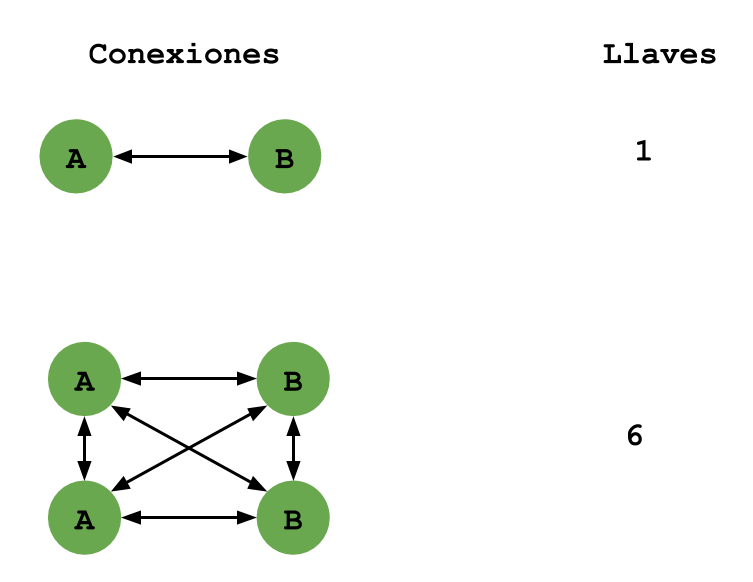
\includegraphics[width=0.65\textwidth]{Llaves}
            \end{figure}

            Ahora si queremos ser mas general es que:
            \begin{MultiLineEquation*}{3}
                llaves\_para\_n\_conexiones(n) 
                    &= \dfrac{n(n-1)}{2}
            \end{MultiLineEquation*}

            Por ejemplo para $n = 30$, osea si hay 30 nodos tenemos que:
            \begin{MultiLineEquation*}{3}
                llaves\_para\_n\_conexiones(30) 
                    &= \dfrac{30(29)}{2}   
                    &= 435
            \end{MultiLineEquation*}




% //////////////////////////////////////////////////////////////////////////////////////////////////////////
% ///////////////////                       CLASICA                                /////////////////////////
% //////////////////////////////////////////////////////////////////////////////////////////////////////////
\part{Clásica}

    % ===============================================================================
    % =====================      IDEAS GENERALES       ==============================
    % ===============================================================================
    \chapter{Ideas generales}

        \begin{itemize}
            \item En general, el alfabeto cifrado esta en minusculas y el alfabeto cifrado esta en mayuscula
        \end{itemize}

    % ===============================================================================
    % =====================      SUSTITUCION           ==============================
    % ===============================================================================
    \chapter{Historia}

        % =========================================================
        % =======               PORQUE             ===============
        % =========================================================
        \clearpage
        \section{Porque es importante cifrar la información}

            
            En general ciframos mensajes porque queremos que estos no caigan en las manos
            del enemigo, ademas para proteger el mensaje de tal manera que solo ciertos sectores
            de la poblacion tuvieran acceso a estos.

            En la mañana del sábado 15 de octubre de 1586, la reina María entró en la concurrida sala
            del tribunal en el castillo de Fotheringhay. 

        % =========================================================
        % =======               PORQUE             ===============
        % =========================================================
        \clearpage
        \section{Cifrado y Mary}

            Mary Queen of Scots fue juzgada por traición. Había sido acusada de conspirar para asesinar a la
            reina Isabel con el fin de llevarse la corona inglesa. Sir Francis Walsingham, secretario
            principal de Elizabeth, ya había arrestado a los otros conspiradores, extrajo confesiones
            y las ejecutó. Ahora planeaba probar que Mary estaba en el corazón de la trama y, por lo
            tanto, era igualmente culpable e igualmente merecedora de muerte.
        
        % =========================================================
        % =======               ROSETTA             ===============
        % =========================================================
        \clearpage
        \section{La piedra Rosetta}

            Encontrada en la época de Napoleon, durante sus campañas por Egipto, cuando la descubrieron 
            se dieron cuenta que tenia un mensaje escrito en 3 lenguas diferentes, usando el griego, que era
            conocido para poder descifrar los jeroglificos.
            
            Esto se realizo en 1820 por Jean Francois.

        % =========================================================
        % =======               ENIGMA SUECO        ===============
        % =========================================================
        \clearpage
        \section{Enigma Sueco}

            El creador fue Boris Hagelin en Suecia, Estocolmo, era una alternativa a la maquina enigma, 
            era considera mas segura, aunque en el fondo no lo era.

            Tambien se creo una version (C-35) que podia caber en un bolsillo.

        % =========================================================
        % =======               ENIGMA SUECO        ===============
        % =========================================================
        \clearpage
        \section{Maquina Purpura}

            Fue creada por Japon, y fue apodada por los descrifradores como la maquina purpura.
            Fue descrifra por los estadounidenses en un par de meses, de hecho lograron hacer una maquina que automatica
            descifrara mensaje.


        % =========================================================
        % =======               GRANDES PERSONAJES       ==========
        % =========================================================
        \clearpage
        \section{Grandes personajes}

            % =========================================================
            % =======               ALAN TURING              ==========
            % =========================================================
            \subsection{Alan Turing}

                \begin{wrapfigure}{r}{0.35\textwidth}
                    \centering
                    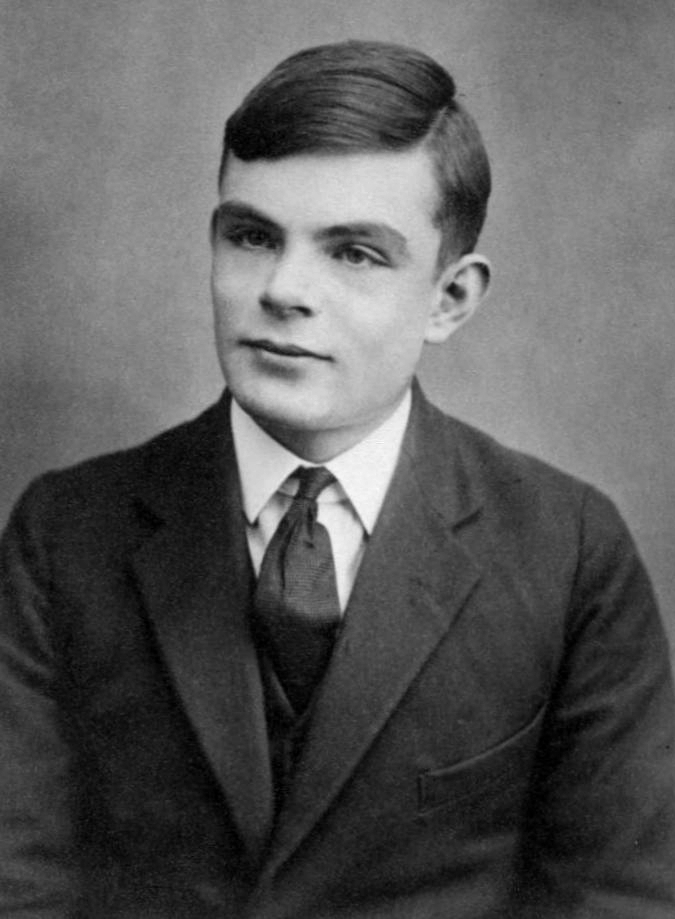
\includegraphics[width=0.30\textwidth]{Turing}
                \end{wrapfigure}

                Alan Turing fue concebido en Chatrapur, India, y nació el 23 de junio de 1912 en Londres,
                mientras sus padres pasaban una temporada de descanso en su tierra natal.

                Cuando tenía solo un año de edad, sus padres regresaron a la India por unos años más,
                y a él y a su hermano mayor los dejaron al cuidado de un coronel del ejército retirado
                y su esposa para que los criaran en una ciudad costera del sur de Inglaterra. 
                
                En su último año en Sherborne, Turing obtuvo una beca para asistir al King’s College de 
                Cambridge, en el que ingresó en 1931 para cursar estudios de matemáticas. 
                
                ...En un congreso celebrado en 1928, Hilbert planteó tres preguntas fundamentales
                válidas para cualquier sistema formal de matemáticas: 

                \begin{itemize}
                    \item 
                        ¿Era su conjunto de reglas completo, de modo que cualquier enunciado pudiera 
                        demostrarse (o refutarse) utilizando solo las reglas del propio sistema?
                    \item 
                        ¿Era coherente, de modo que ningún enunciado pudiera demostrarse verdadero y a la vez falso?
                    \item 
                        ¿Existía algún procedimiento que pudiera determinar si un enunciado concreto 
                        era demostrable, en lugar de permitir la posibilidad de que algunos enunciados 
                        (como les ocurría a problemas muy famosos, como el teorema de Fermat,
                        la conjetura de Goldbach o de Collatz)? 
                \end{itemize}
                
                Hilbert pensaba que la respuesta a las dos primeras preguntas era que sí, 
                por lo que no tenía mucho sentido hacerse la tercera. 

                Cuando el gran profesor de matemáticas de Cambridge Max Newman le
                enseñó a Turing las preguntas de Hilbert, el expresó el Entscheidungsproblem
                del siguiente modo: ¿Existe algún proceso mecánico que se pueda utilizar para determinar
                si un enunciado lógico concreto es demostrable?

                A Turing le gustó el concepto de proceso mecánico.
                En 1937 Alan Turing publicaba \Quote{Sobre los números computables}, en el que
                describe un computador universal, resolviendo la tercera pregunta de Hilbert.

                En su intento de identificar preguntas indecidibles, el artículo de Turing
                describió una máquina imaginaria que fue diseñada para realizar una operación
                matemática o algoritmo particular. 
                
                En otras palabras, la máquina sería capaz de ejecutar una serie de pasos fijos y prescritos que,
                por ejemplo, multiplicarían dos números.
                
                Turing preveía que los números que se multiplicarían podrían introducirse en la máquina a
                través de una cinta de papel, como la cinta perforada que se utiliza para alimentar una
                melodía en una piano antiguo. 
                La respuesta a la multiplicación se emitirá a través de otra cinta.
                Turing imaginó una serie completa de estas llamadas máquinas de Turing,
                cada una especialmente diseñada para abordar una tarea en particular,
                como dividir, cuadrar o factorizar.

                Luego dio el siguiente paso. Se imaginó una máquina cuyo funcionamiento interno
                podría ser alterado para que pudiera realizar todas las funciones de todas las
                máquinas de Turing concebibles. Las modificaciones se realizarían insertando
                cintas cuidadosamente seleccionadas, que transformaron la máquina flexible
                individual en una máquina divisoria, una máquina multiplicadora o cualquier
                otro tipo de máquina. Turing llamó a este dispositivo hipotético una máquina
                universal de Turing porque sería capaz de responder cualquier pregunta que
                pudiera ser respondida lógicamente.

                En otras palabras Turing pensó: 
                \Quote{No necesitamos una infinita variedad de máquinas distintas que realicen 
                tareas diferentes. Bastará con una sola. 
                
                Del problema técnico de crear máquinas distintas para diversas tareas se pasa a la 
                labor administrativa de “programar” la máquina universal para llevar a cabo esas tareas}

                La carrera académica de Turing se detuvo abruptamente unos años mas tarde
                cuando gracias al \Quote{Government Code and Cypher School} fue invitado a convertirse en
                criptoanalista en Bletchley, justo el 4 de septiembre de 1939,
                el día después de que Neville Chamberlain declarara la guerra a Alemania

                Turing comenzó a trabajar en la decodificación de la máquina The Enigma, 
                un dispositivo de cifrado desarrollado y utilizado a principios y mediados del
                siglo XX utilizado por la Alemania nazi para proteger la comunicación comercial,
                diplomática y militar.

                Turing se centró en lo que sucedería si el ejército alemán cambiara su sistema
                de intercambio de claves de mensajes.
                
                Los primeros éxitos de Bletchley se basaron en el trabajo de Rejewski, que explotó el hecho de
                que los operadores de Enigma cifraron cada clave de mensaje dos veces
                (por ejemplo, si la clave de mensaje era YGB, el operador cifraría YGBYGB).
                Se suponía que esta repetición aseguraría que el receptor no cometiera un error, pero creó
                una brecha en la seguridad de Enigma.  

                Los criptoanalistas británicos adivinaron que no
                pasaría mucho tiempo antes de que los alemanes se dieran cuenta de que la clave repetida
                estaba comprometiendo a Enigma, en cuyo punto se les pediría a los operadores
                de Enigma que abandonaran la repetición, confundiendo así las técnicas actuales de descifrado de
                códigos de Bletchley. (Simon Singh, The Code Book Book, Chapter 4: Enigma)
                
                Era el trabajo de Turing encontrar una forma alternativa de atacar a Enigma,
                una que no dependiera de una clave repetida.

                Esta sería la semilla de una máquina electromecánica llamada bombe (que le tomo un par de semanas), 
                que podría romper Enigma de manera más efectiva que la bomba kryptologiczna polaca.

                Se ha argumentado, aunque de forma controvertida, que los logros de Bletchley Park 
                fueron el factor decisivo en la victoria de los aliados.
                
                Lo que es seguro es gracias a los trabajos de Bletchley se
                acortó significativamente la guerra.
                
                Esto se hace evidente al pensar en la situación en la Batalla del Atlántico
                y especular sobre lo que podría haber sucedido sin el beneficio de Ultra.
                
                Para empezar, se habrían perdido más barcos y suministros para la flota dominante de
                submarinos, lo que habría comprometido el vínculo vital con Estados Unidos y forzado
                a los Aliados a desviar mano de obra y recursos en la construcción de nuevos barcos.
                
                Los historiadores han estimado que esto habría retrasado los planes aliados en varios meses,
                lo que habría significado posponer la invasión del Día D hasta al menos el año siguiente.
                
                Según Sir Harry Hinsley, \Quote{la guerra, en lugar de terminar en 1945, habría terminado en 1948
                si el Reino Unido no hubieran podido leer los cifrados Enigma
                y producir Ultra}
               
                (Walter Isaacson. Innovadores (Innovators-SP)).


            % =========================================================
            % =======               CLAUDE SHANNON           ==========
            % =========================================================
            \subsection{Claude Shannon}

                \begin{wrapfigure}{r}{0.35\textwidth}
                    \centering
                    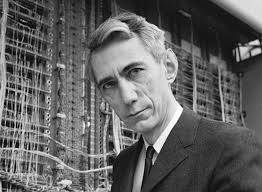
\includegraphics[width=0.30\textwidth]{Shannon}
                \end{wrapfigure}


                En 1937 se produjo otro avance teórico trascendental, 
                similar al de Turing en cuanto que se trataba puramente de un experimento mental.
                Era el trabajo de un estudiante de posgrado del MIT llamado Claude Shannon,
                que aquel año se convirtió en la tesis de máster más influyente de todos los tiempos,
                un artículo que Scientific American calificaría más tarde como: la Carta Magna de la era
                de la información.

                Shannon creció en una pequeña población de Michigan, donde construyó maquetas de
                aviones y aparatos de radioaficionado; luego cursó estudios especializados de
                ingeniería eléctrica y matemáticas en la Universidad de Michigan.

                Si la teoría de la información y la comunicación fueran tan emocionantes
                como la computación y la inteligencia artificial, tal vez Claude Shannon sería tan
                famoso como Alan Turing. 
                
                De hecho, al considerar la totalidad del trabajo de Shannon, puede que no sea una
                exageración decir que fue el padre de la era de la información en la que nos encontramos hoy.
                
                Shannon es mejor conocido por introducir el concepto de entropía como una medida de información.
                
                Esta idea fue introducida por primera vez por Shannon en un informe clasificado escrito para
                Bell Laboratories en 1945 titulado Una teoría matemática de la criptografía.
                El informe fue desclasificado y publicado en el Bell System Technical Journal en 1949
                bajo el título de Communication Theory of Secrecy Systems, 
                un año después de que Shannon publicara su artículo A Mathematical Theory of Communication.

                Había una dualidad entre Shannon y Turing y su trabajo de criptografía en los tiempos de guerra.
                
                Mientras Turing estaba en Bletchley Park decodificando mensajes interceptados de los alemanes,
                proporcionando a Churchill información invaluable,
                Shannon estaba en Bell Laboratories trabajando en el Sistema X, 
                un teléfono utilizado por Churchill y Roosevelt para conducir conferencias transoceánicas. 
                
                Shannon estaba trabajando en ocultar información por un lado mientras intentaba
                transmitirla por otro lado, y tuvo la idea de su teoría de la comunicación mientras
                trabajaba en el esquema de cifrado para el Sistema X. 
                
                \Quote{Se dio cuenta de que, así como los códigos digitales podían proteger la información
                de miradas indiscretas, también podían protegerla de los estragos de la interferencia
                estática u otras formas de interferencia}. (Horgan, 1992, p. 74).
                
                Al trabajar en su documento de criptografía de 1945, Shannon se dio cuenta de que los códigos digitales
                podrían diseñarse para empaquetar información no solo de manera más eficiente 
                (de modo que se pudiera transmitir más información a través de un canal dado), 
                sino que también podrían diseñarse para hacerlos irrompibles. (Shannon, 1949) 
                
                Mientras que en la criptografía desea proteger un mensaje de espías, 
                en la información desea proteger un mensaje de errores de transmisión. 
                En ambos campos se necesita una medida de información y se trabaja con métodos de
                codificación y decodificación
                
                Resultó que ambos implicaban lo mismo, la entropía, que se convertiría en la pieza clave de la
                teoría de la información de Shannon.

                {\large
                Cuando Von Neumann murió, dejando su volumen\Quote{
                    The Computer and the Brain} sin terminar
                solo había dos nombres mencionados en todo el libro: Alan Turing y Claude Shannon.}



    

    % ===============================================================================
    % =====================      SUSTITUCION           ==============================
    % ===============================================================================
    \chapter{Sustitución}

        Es tomar cada caracter del alfabeto y transformarlo en otro diferente, cada caracter
        siempre va a parar al mismo caracter.

        % =========================================================
        % =======               DECIMAL             ===============
        % =========================================================
        \clearpage
        \section{Cifrado Cesar y de corrimiento}

            Creado por el famoso general griego Cesar, el método es hacer un corrimiento del alfabeto, por ejemplo con un $k=3$, 
            entonces $A \to D$ ó $B \to E$.

            Otra versión del cifrado tomaba el alfabeto griego y lo transformaba por el romano.

            La fórmula general es:
            \begin{MultiLineEquation*}{3}
              e(x) = x + k \Space mod 26  
            \end{MultiLineEquation*}
            

        % =========================================================
        % =======               AFFINE              ===============
        % =========================================================
        \clearpage
        \section{Cifrado Affine}

            Es parecido al de corrimiento, se puede escribir como:
            
            \begin{MultiLineEquation*}{3}
                e(p) &= \alpha p + \beta \\
                d(c) &= \alpha^{-1} (p - \beta)
            \end{MultiLineEquation*}


        % =========================================================
        % =======               DECIMAL             ===============
        % =========================================================
        \clearpage
        \section{Cifrado Vigenène}
            
            Es un cifrado de sustitución polialfabetico, porque una misma letra en el mensaje en texto plano sera mandado a diferentes
            letras dependiendo de su posicion en el mensaje original. 

            Su fórmula general:
            \begin{MultiLineEquation*}{3}
                E_k(M_i) = (M_i + K_i) \Space mod L  
            \end{MultiLineEquation*}

            \begin{MultiLineEquation*}{3}
                D_k(C_) = (C_i - K_i) \Space mod L  
            \end{MultiLineEquation*}

            \begin{itemize}
                \item Primero que nada, escribe el mensaje en texto plano
                \item Se usa una llave que se escribe tantas veces como sea necesario
                \item Se busca en la tabla 
            \end{itemize}




        
    % ===============================================================================
    % =====================      TRANSPOSICION         ==============================
    % ===============================================================================
    \chapter{Transposicion}

    % ===============================================================================
    % =====================      SUSTITUCION           ==============================
    % ===============================================================================
    \chapter{Cripto analisis}


        % =========================================================
        % =======               DECIMAL             ===============
        % =========================================================
        \clearpage
        \section{Analisis de Frecuencias}

            No es loco pensar que la letra que mas aparece en un mensaje cifrado sera la letra mas comun
            del alfabeto original.


            

% //////////////////////////////////////////////////////////////////////////////////////////////////////////
% ///////////////////                       MODERNA                                /////////////////////////
% //////////////////////////////////////////////////////////////////////////////////////////////////////////
\part{Moderna}


    % ===============================================================================
    % =====================      LLAVE PUBLICA         ==============================
    % ===============================================================================
    \chapter{De llave privada o simétrica}

        % =========================================================
        % =======               FLUJOS              ===============
        % =========================================================
        \clearpage
        \section{Flujos}

        % =========================================================
        % =======              BLOQUES              ===============
        % =========================================================
        \clearpage
        \section{Bloques}

        
    % ===============================================================================
    % =====================      LLAVE PRIVADA         ==============================
    % ===============================================================================
    \chapter{De llave pública o asimétrica}





                
% ===============================================
% ========        BIBLIO      ===================
% ===============================================
\begin{thebibliography}{10}

  \bibitem{Udacity} 
    Nidia A. Cortez-Duarte, Cryptography
      \textit{2019}. 

  \bibitem{Innovators} 
    Walter Isaacson. “Innovadores (Innovators-SP).

\end{thebibliography}


\end{document}